\documentclass[tikz,border=8pt]{standalone}
% Shared look for every TikZ diagram. Load with \input{../../tools/tikz-style.tex}
\usepackage[T1]{fontenc}
\usepackage{lmodern}
\renewcommand{\sfdefault}{lmr}  % diagrams use the same serif as the text
\usetikzlibrary{arrows.meta, positioning, shapes.geometric, calc, fit, backgrounds}
\definecolor{cblue}{HTML}{4C78A8}
\definecolor{corange}{HTML}{F58518}
\definecolor{cgreen}{HTML}{54A24B}
\definecolor{cred}{HTML}{E45756}
\definecolor{cpurple}{HTML}{B279A2}
\definecolor{cgrey}{HTML}{6B6B6B}
\tikzset{
  every picture/.style={font=\sffamily, line width=1.2pt},
  box/.style={draw=#1, fill=#1!12, rounded corners=4pt, align=center, inner sep=7pt, minimum height=1.1cm},
  box/.default=cgrey,
  arrow/.style={-{Stealth[length=3mm]}, draw=cgrey, line width=1.4pt},
  title/.style={font=\sffamily\bfseries\Large},
  note/.style={font=\sffamily\small, text=cgrey, align=center},
}
\AtBeginDocument{\hyphenpenalty=10000 \exhyphenpenalty=10000}

\begin{document}
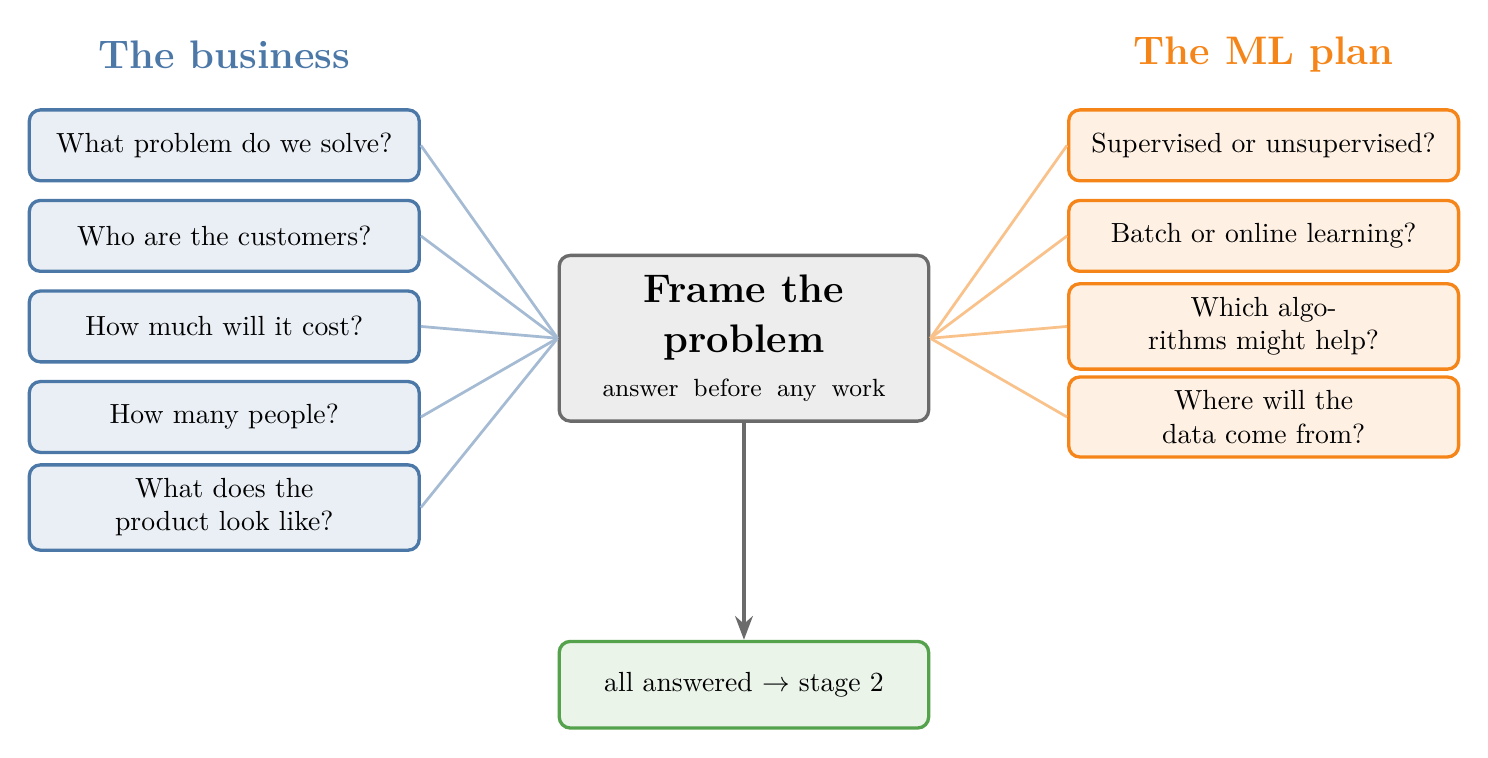
\begin{tikzpicture}[q/.style={box=#1, text width=4.6cm, minimum height=0.9cm, inner sep=5pt, font=\sffamily}]
  \node[box=cgrey, font=\sffamily\bfseries\Large, text width=4.2cm] (c) at (0,0) {Frame the problem\\[-2pt]\normalfont\small answer before any work};
  % business questions (left)
  \node[title, text=cblue] at (-6.6,3.6) {The business};
  \foreach \t [count=\i] in {What problem do we solve?, Who are the customers?, How much will it cost?, How many people?, What does the product look like?}
    \node[q=cblue] (b\i) at (-6.6,3.6-1.15*\i) {\t};
  % ML questions (right)
  \node[title, text=corange] at (6.6,3.6) {The ML plan};
  \foreach \t [count=\i] in {Supervised or unsupervised?, Batch or online learning?, Which algorithms might help?, Where will the data come from?}
    \node[q=corange] (m\i) at (6.6,3.6-1.15*\i) {\t};
  \foreach \i in {1,...,5} \draw[cblue!50, line width=1pt] (c.west) -- (b\i.east);
  \foreach \i in {1,...,4} \draw[corange!50, line width=1pt] (c.east) -- (m\i.west);
  \node[box=cgreen, text width=4.2cm, font=\sffamily] (go) at (0,-4.4) {all answered $\to$ stage 2};
  \draw[arrow] (c) -- (go);
\end{tikzpicture}
\end{document}
